\documentclass[oribibl]{llncs}
\usepackage{graphicx}
\graphicspath{ {Figures/} }

\begin{document}

\title{SNARC - An Approach for Aggregating and Recommending Contextualized Social Content} 
\author{Ahmad Assaf\inst{1} \and Aline Senart\inst{1} \and Raphael Troncy\inst{2}} 
\institute{SAP Research, SAP Labs France SAS,\\
805 avenue du Dr. Maurice Donat, BP 1216, 06254 Mougins Cedex, France
\email{first.last@sap.com}
\and
EURECOM,\\
2229 route des cretes, 06560 Sophia Antipolis, France\\
\email{raphael.troncy@eurecom.fr}}
\maketitle

\begin{abstract}
The Internet has created a paradigm shift in how we consume and disseminate information. Data nowadays is spread over heterogeneous silos of archived and live data. People willingly share data on social media by posting news, views, presentations, pictures and videos. SNARC is a service that uses semantic web technology and combines services available on the web to aggregate social news. SNARC brings live and archived information to the user that is directly related to his active page. The key advantage is an instantaneous access to complementary information without the need to dig for it. Information appears when it is relevant enabling the user to focus on what is really important.
\keywords{Social news, social networks, aggregator, data mining, mashup}
\end{abstract}

\section{Introduction}
With the rapid advances of the Internet, social media become more and more intertwined with our daily lives. The ubiquitous nature of Web-enabled devices, especially mobile phones, enables users to participate and interact in many different forms like photo and video sharing platforms, forums, newsgroups, blogs, micro-blogs, bookmarking services, and location-based services. Social networks are not just gathering Internet users into groups of common interests, they are also helping people follow breaking news, contribute to online debates or learn from others. They are transforming Web usage in terms of users' initial entry point, search, browsing and purchasing behavior.\cite{Bakshy2012}
A common scenario that often happens while reading an interesting article, coming across a nice video or participating in a discussion in a forum is the growing interest to check related material around the information read. To do so, users might go to Twitter\footnote{http://www.twitter.com}, Google+\footnote{http://plus.google.com}or YouTube\footnote{http://www.youtube.com}. They can try several times with several keywords to obtain the desired results. In the end, they might end up with several browser tabs opened and get distracted by the information overload from all these resources. The same happens in companies when business users are interested in information provided by corporate web applications like enterprise communities. SNARC is a semantic social news aggregator that leverages live rich data that social networks provide to build an interactive rich experience on the Internet. The service retrieves news related to the current page from popular platforms like Twitter, Google+, YouTube, Vimeo\footnote{http://www.vimeo.com}, Slideshare\footnote{http://www.slideshare.com}, Stackoverflow\footnote{http://www.stackoverflow.com}and the Web. As a possible front-end implementation, we have created a Google Chrome extension (visit http://ahmadassaf.com/SNARC) which enriches the user experience by augmenting related contextual information to entities on the page itself, as well as displaying related social news on a floating sidebar. 
\\The remainder of this paper is split into three main sections. The first talks about the underlying mechanism of the service, splitting the functionalities into three main subsections. The second describes the front-end implementation, and the last talks about our conclusion and future work.

\section{Underlying Mechanism}
The back-end of SNARC consists of three major components: a document handler that creates a "Semantic Model" that represents any web resource, a query layer that is responsible for disseminating queries to the supported social services and a data parser which processes the search results, wraps them in a common social model and generates the desired output.

\subsection{Document Handler}
The main idea behind SNARC is to provide a uniform model for web entities, whether they are blog entries, multimedia objects or micro-posts. To do so, SNARC creates a "Semantic Model" containing all the annotations and meta-data needed to query and reconcile social results. 
\begin{figure}[h!]
  \centering
    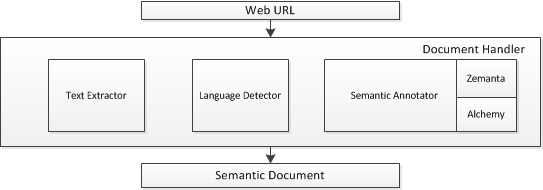
\includegraphics[scale=0.8]{architecture-part1.png} 
  \caption{SNARC's Document Handler}
\end{figure}

The Semantic Model is created by the Document Handler (see Figure 1) which receives a web page URL and performs these three main steps:
\begin{enumerate}
\item {\bf Text Extraction:} Fetch the webpage that corresponds to the received URL and extract the textual content using a set of heuristics. These latter identify the main content of the page by stripping unwanted HTML tags and rank the different sections based on their semantics, class names and order. In the beginning we have used Alchemy API\footnote{http://www.alchemyapi.com} to perform text extraction; but we have chosen to implement a simpler method ourselves which saved us an extra API call. 
\item {\bf Language Detection:} Detect the web page language using the Language Detection service of Alchemy API. This is necessary to match the desired language with compatible services like Twitter, YouTube, etc.
\item {\bf Semantic Annotation:} Annotating the extracted text is the most important step in this process. We use Zemanta Suggest\footnote{http://developer.zemanta.com/docs/suggest/} and Alchemy API in order to extract: 
\begin{itemize}
\item {\bf Tags:} These are the finest-grained queryable "keywords" that we use to retrieve the social results. From our experiments, combining tags results in better findings than using entities or concepts. However, we plan to evaluate the combination of keywords, entities and concepts in order to find the top-queryable terms that will retrieve the most relevant results on different abstraction levels.
\\Tags retrieved from these services are ranked by confidence values calculated by their internal algorithms, these values are normalized for each service. According to our experiments we have found that Alchemy's Keywords Extraction API returns a large set of closely related keywords (i.e. Android, Android Phone, Android Tablet, ...). To construct a good query we therefore need to provide a certain level of abstraction.We perform a cleaning process on those keywords by applying the Levenshtein distance to rule out closely related keywords by disregarding those with lower confidences. We perform a similar process on the result of the union between the keywords returned by Alchemy and Zemanta to ensure a sparse keywords set.
\item {\bf Semantic Entities:} Entities provide a higher abstraction level of the document. They are used to reconcile the social results in order to maintain relevancy with the document. Similar to the keywords extraction services, the entities retrieved are ranked and contain outbound links to the matched entity on dbpedia, Wikipedia, Freebase, etc. A union is made between the results from Alchemy and Zemanta to ensure a wider coverage of entities. When a match is found, we merge the links from the two sources to ensure that we include all the resources that can be used to augment extra information about that entity in the document. 
\item {\bf Categories:} These are high-level taxonomies that can generally describe the document's content. A taxonomy is used to narrow down our query scope when targeting services like YouTube. In our Semantic Document model we define two possible category sets, one retrieved from Alchemy's Text Categorization API\footnote{http://www.alchemyapi.com/api/categ/categs.html} and the other retrieved from Zemanta Suggest API that follows the DMOZ categorization scheme\footnote{http://www.dmoz.org/desc/Top}.
\end{itemize}
\end{enumerate}
At the end of this process, we will have constructed the needed elements (keywords, entities and high level categories) wrapped in our Semantic Model to be passed to the query generator. For example, a summary of the Semantic Model for a web page titled "Turkey protests: Erdogan in 'final' warning\footnote{http://www.bbc.co.uk/news/world-europe-22889060}"  looks like: 
\begin{enumerate}
\item {\bf Categories:} Culture\_Politics, Regional and Society
\item {\bf Keywords:} Taksim Square, Protesters, Gezi Park, Mr Erdogan, Istanbul ...
\item {\bf Entities:} Gezi Park, Recep Tayyip Erdogan, Taksim Square, Justice and Development Party (Turkey), Police of Turkey ...
\end{enumerate}

\subsection{Query Layer}
In this component, the calls to the social services are made. SNARC uses the extracted keywords from the Semantic Document in order to construct the queries and disseminate them to the appropriate services. Figure 2 shows the different steps in order to retrieve a set of social results.
\begin{figure}[h!]
  \centering
    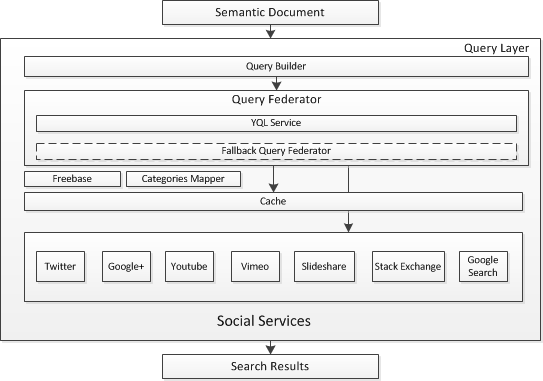
\includegraphics[scale=0.75]{architecture-part2.png}
  \caption{SNARC's Query Layer}
\end{figure}

\begin{enumerate}
\item {\bf Query Builder:} Responsible for identifying targeted services and building tailored queries for each service. For example, if the processed document is categorized as a computer or technology related one, Stackoverflow service will be targeted with the queries constructed. However, other categories will correspond to different services from the Stack Exchange websites\footnote{http://stackexchange.com/sites}.
\item {\bf Query Federator:} Responsible for federating the queries identified in the previous step to the corresponding services. To enhance performance, we tried to reduce the number of external calls. Yahoo Query Language (YQL)\footnote{http://developer.yahoo.com/yql/} helped us in minimizing the number of calls and batching them into a single one. It is an expressive SQL-like language that lets you query, filter, and join data across Web services. However, we have found that we cannot fully rely on YQL due to their API calls limit and the restriction on the query execution time that is set to 30 seconds. To overcome this, we have implemented a fallback mechanism that federates the queries to the selected social services and groups the result to be passed afterwards to the parser. \\
To further optimize the number of calls, we have decided to take the top two ranked keywords. We do not apply logical operator (AND/OR) in our queries; instead, we perform one-to-one mapping between each keyword and query. Indeed, we have found that gathering keywords even if semantically related might bring up noise in the results. However, as mentioned earlier, a part of the future work will be investigating the best method to construct the most relevant queryable entity using different logical operators.
\item {\bf Caching:}The main setback in the query layer was the variable limited number of calls we can make to external APIs. To overcome this, we have implemented a simple cache mechanism that saves the results on disk up to an hour. There are several cache levels; the first is a URL level one where the results of the parsed queries are cached. For example, if a user visited a certain article on the CNN webpage the results might take up to 15 seconds to appear, whereas a second user visiting the same article minutes afterwards will have the cached results in few seconds. The second level is keyword and service specific. This can be very helpful as users generally browse articles of related topics or interests (semantic concepts), so for each user we can end up with the same high level concepts being requested frequently. An important thing to note is that the caching is done on the server side and is disk-based.
\end{enumerate}
The social services queried can be grouped as follows:
\begin{enumerate}
\item {\bf Multimedia Services:} They include Slideshare, Vimeo and YouTube. Slideshare and YouTube allow the results to be fetched in a specific language that was detected in the previous step. In addition to that, YouTube search services are called twice; the first call is done to the YouTube V2 API\footnote{https://developers.google.com/youtube/2.0/} where we specify in addition to the keywords a high level category to be targeted. To do so, we have manually created a category mapping file that maps the high-levels categories of Alchemy’s API and DMOZ to those provided by YouTube. The second call is done to YouTube V3 API\footnote{https://developers.google.com/youtube/v3/}. The new feature provided by Google in this version is the ability to search using a semantic concept that corresponds to a Freebase concept ID; it proves to retrieve better results that the normal search. Freebase concept calls are cached for longer periods as they are less prone to changes. 
\item {\bf Micro-posts Services:} They include Twitter, Google+ and Stackoverflow. Language filtering is done where applicable. 
\item {\bf General Search:} This includes similar results found via Google search or those retrieved from the Zemanta API call. They are general articles or blog posts related to the current active page.
\end{enumerate}
\subsection{Data Parser}
This is the last step where the results and unified and wrapped in a single social model. Figure 3 shows the different steps needed to produce the final parsed results that will be pushed back to the front-end.
\begin{figure}[h!]
  \centering
    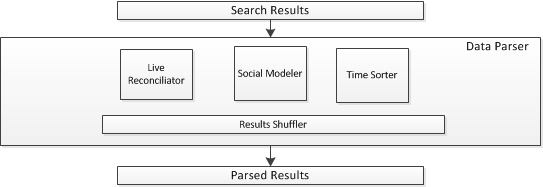
\includegraphics[scale=0.8]{architecture-part3.png} 
  \caption{SNARC's Data Parser}
\end{figure}

\begin{enumerate}
\item {\bf Live Reconciliator:} Social (or folksonomic) tagging has become a trending method to describe, search and discover content on the web. Folksonomies empower users by giving them total freedom in choosing their categories and keywords that they think describe best the content. This contrasts with taxonomies that over-impose hierarchical categorization of content \cite{Zanardi2008}. However, in services like Twitter and Google+, tagging has been abused in a way that increased noise in the stream of results. To overcome this problem, we align the incoming stream of posts with the set of semantic concepts or keywords that describe the document. There are several approaches and tools like \cite{Cantador2011,Diaz-Aviles2012,Preotiuc-Pietro2012,Zanardi2008} that aim at solving this problem. In SNARC we rely on two levels of reconciliation: one uses the high-level taxonomy (categories); and the other uses the vector of entities defined in the Semantic Document. For example, if SNARC wants to reconcile a blog post result retrieved from a general search, it constructs a Semantic Document Model for that result and applies the Cosine Similarity on the vector of ranked entities for each Semantic Model. Currently, we only reconcile against blog posts as it is very straightforward to construct a Semantic Document Model for them. However, an integral part of the future work will be the integration of SNARC's model to micro-posts and video search services.

\item {\bf Social Modeler:} Every social network has its own underlying data model. To overcome this problem, we need to present the social results in a common wrapper. To do so, we have created an optimized universal social model that contains all the necessary data to model social information and can be reused in other projects. The model contains service related attributes like the service name and type, general post information like the author's name, profile link, image and geo-location information and post-specific information like the title, thumbnail, embed code, main content and link. 
\item {\bf Time Sorter and Results Shuffler:} To better display the results on the front-end, we unify the time representation and sort the results based on it. Afterwards we pick the top N results and shuffle them to generate a random order.
\end{enumerate}

\section{Front-End}
SNARC is a service that generates a JSON file containing the results wrapped in our universal social model. We have implemented a chrome extension that loads SNARC on any web page or application (see Figure 4). This UI implementation offers more flexibility to users by loading related social news anytime on any webpage or application. The results are visualized using jQuery templates as a sliding panel on one of the screen edges, extracted entities are highlighted in the page itself and a short excerpt is displayed when hovering over them.
\begin{figure}[h!]
  \centering
    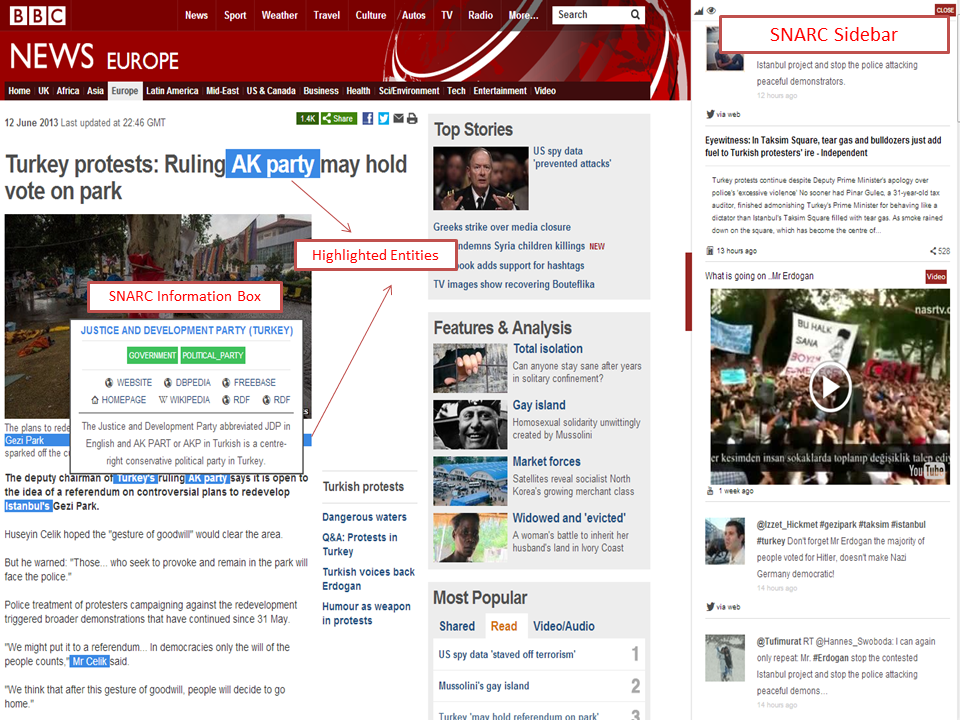
\includegraphics[scale=0.45]{SNARC-annotated.png} 
  \caption{SNARC's UI - The Google Chrome Extension}
\end{figure}


\section{Conclusions and Future Work}
Aggregating relevant social news is not an easy task. SNARC performs the task in a nice and intuitive way that allows the user to discover what is happening instantly and without the need to navigate away from the current page. One of the important things to consider for the future is the integration of better reconciliation features and tools to ensure the display of relevant social posts. Moreover, real-time feature that can also push new related posts would be a great addition. We would also want to test SNARC on business web applications. It can be a good fit to perform brand monitoring especially after plugging a sentiment analysis component. We would also like to evaluate the necessity to use a content scrapping API like Alchemy’s as a fallback for our text extraction mechanism.

\bibliographystyle{abbrv}
\bibliography{SNARC}


\end{document}


